\documentclass[tikz]{standalone}
\usetikzlibrary{calc,trees,positioning,arrows,chains,shapes.geometric,%
    decorations.pathreplacing,decorations.pathmorphing,shapes,%
    matrix,shapes.symbols,fit}

\pgfdeclarelayer{back}
\pgfsetlayers{back,main}


\makeatletter
\tikzset{
  fitting node/.style={
    inner sep=0pt,
    fill=none,
    draw=none,
    reset transform,
    fit={(\pgf@pathminx,\pgf@pathminy) (\pgf@pathmaxx,\pgf@pathmaxy)}
  },
  reset transform/.code={\pgftransformreset}
}
\makeatother


\begin{document}
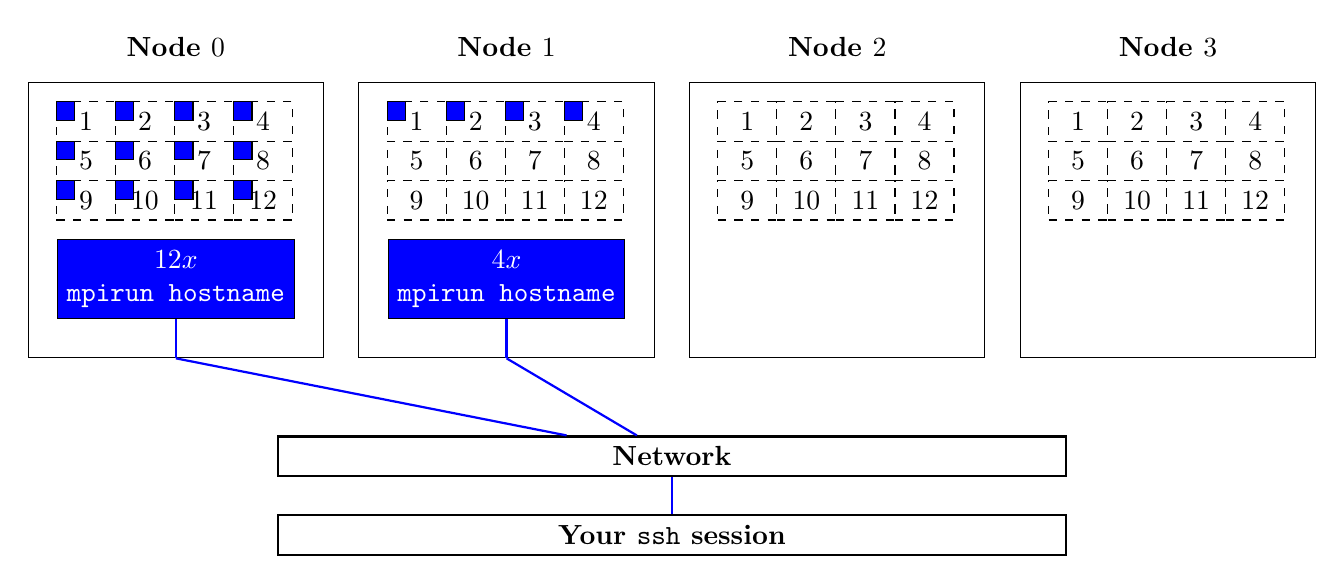
\begin{tikzpicture}

  \node [draw,thick,rectangle, minimum width=10cm, minimum height=.5cm] at($(1.5*4.2,0)$) (switch) {\bfseries{}Network};
  \node [draw,thick,rectangle, minimum width=10cm, minimum height=.5cm] at($(1.5*4.2,-1)$) (you) {\bfseries{}Your \texttt{ssh} session};
  \path [thick,color=blue] (switch) edge (you) ;
  
  \foreach \n in {0,...,3}
  {
   
    \node [draw,rectangle, minimum width=3.75cm, minimum height=3.5cm] at($(0,3)+(4.2*\n,0)$) (node_\n) {};
    \node [node distance=2mm,above =of node_\n] (node_label_\n) {\bfseries{}Node $\n$};
    \node [below] (cpus_\n) at($(node_\n.north)+(-1.4,-.25)$)  {};

    \foreach \y in {0,...,2}{
      
      \foreach \x in {0,...,3}{
        \pgfmathsetmacro\result{(\y * 4 + \x)+1}
        \node [draw,dashed,rectangle,minimum width=.75cm,minimum height=.5cm,anchor=north west] at($(cpus_\n.north west)+(\x*.75,\y*-.5)$) (node_\n_core_\x_\y) {\pgfmathprintnumber{\result}};
      
      }
    }


  }

    \node [draw, align=center, above, fill=blue, text=white, minimum height=1cm] at($(node_0.south)+(0,.5)$) (mpirun_call_0) {$12x$\\$\texttt{mpirun hostname}$};
    \path [thick,color=blue] (mpirun_call_0) edge (node_0.south) 
    (node_0.south) edge (switch);

    \foreach \x in {0,...,3}{

      \node [draw,fill=blue,rectangle,minimum width=2mm,minimum height=2mm,anchor=north west] at(node_1_core_\x_0.north west) (busy_1_core_\x) {};

      \foreach \y in {0,...,2}{
        \node [draw,fill=blue,rectangle,minimum width=1mm,minimum height=1mm,anchor=north west] at(node_0_core_\x_\y.north west) (busy_0_core_\x_\y) {};
      }
    }


    \node [draw, align=center, above, fill=blue, text=white, minimum height=1cm] at($(node_1.south)+(0,.5)$) (mpirun_call_1) {$4x$\\$\texttt{mpirun hostname}$};
    \path [thick,color=blue] (mpirun_call_1) edge (node_1.south) 
    (node_1.south) edge (switch)
    (switch) edge (you);

\end{tikzpicture}
\end{document}
